\documentclass[aspectratio=169]{beamer}

\usetheme{Singapore}
\usecolortheme{default}
\setbeamertemplate{navigation symbols}{}
\setbeamertemplate{footline}[frame number]
\setbeamertemplate{itemize items}[circle]
\setbeamerfont{frametitle}{size=\Large}
\setbeamerfont{normal text}{size=\large}
\setbeamercolor{structure}{fg=blue!70!black}

\usepackage{graphicx}
\usepackage{booktabs}
\usepackage{array}
\usepackage{tikz}
\usepackage{hyperref}
\usepackage{multicol}
\usepackage{ragged2e}

\graphicspath{{./assets/}{../pictures/}}

\newcommand{\photo}[1]{\includegraphics[width=0.235\textwidth,height=0.68\textheight,keepaspectratio]{#1}}
\newcommand{\photoWide}[1]{\includegraphics[width=0.46\textwidth,height=0.68\textheight,keepaspectratio]{#1}}
\newcommand{\gridphoto}[1]{\includegraphics[width=0.235\textwidth,height=0.30\textheight,keepaspectratio]{#1}}
\newcommand{\gridphotofive}[1]{\includegraphics[width=0.185\textwidth,height=0.30\textheight,keepaspectratio]{#1}}
\newcommand{\smalllabel}[1]{\scriptsize\textcolor{gray}{#1}}

\title{Student Life}
\subtitle{MScAC Orientation Week}
\author{David Goh — MScAC (Applied Math) 2025--2026}
\date{}

\begin{document}

\begin{frame}
  \titlepage
\end{frame}

\begin{frame}{A bit about me}
  \begin{itemize}
    \item Applied Math Concentration, MScAC 2025--2026
    \item Lived in Singapore and the US
    \item Undergraduate Major: Mathematics
    \item Courses Taken: Machine Learning (CSC2515), Deep Learning Theory (MAT1510), Financial Mathematics (MAT1856), Computational Social Science (CSC2552)
    \item MScAC Internship: Horizon3 AI Labs, Unilever PLC
  \end{itemize}
  Reach out for questions about any of the above experiences at \href{mailto:daveed@cs.toronto.edu}{daveed@cs.toronto.edu}
\end{frame}

\begin{frame}{Where do you live?}
  \begin{columns}[c]
    \column{0.72\textwidth}
      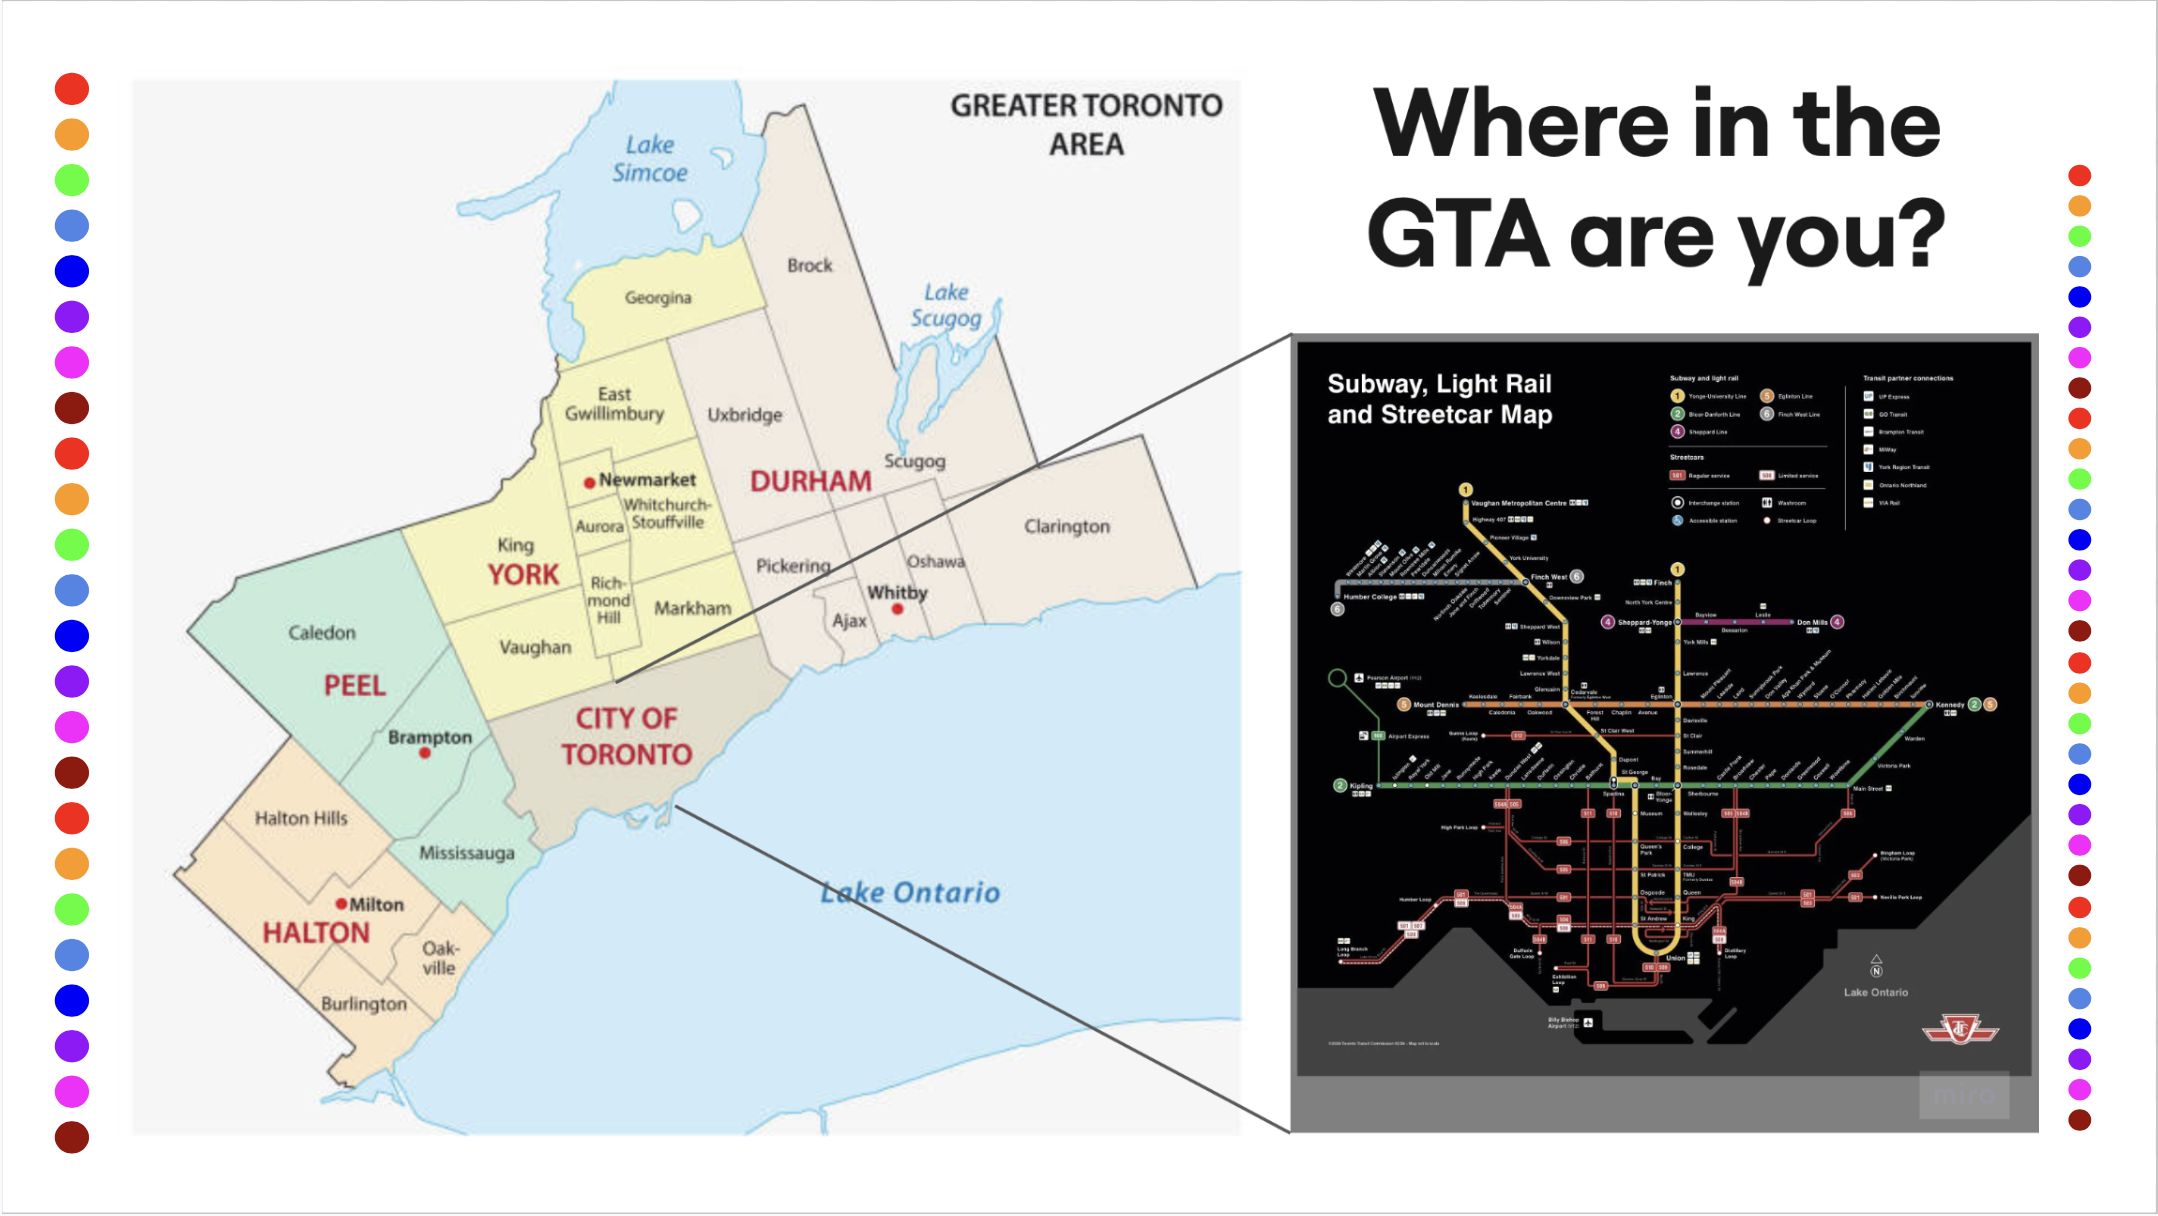
\includegraphics[width=\linewidth,height=0.72\textheight,keepaspectratio]{icebreaker-slide-new.png}
    \column{0.25\textwidth}
      \centering
      
\includegraphics[width=0.8\linewidth]{icebreaker_qr.png}

      \vspace{0.3cm}
      \small Scan the map\\
      \small Add your pin
  \end{columns}
\end{frame}

\begin{frame}{Weekends in Toronto}
  \begin{columns}[T]
    \column{0.32\textwidth}
      \textbf{Explore}\\[0.15cm]
      Parks: High Park, Trinity Bellwoods, Tommy Thompson
      Waterfront: CN Tower, Toronto Islands
      Neighbourhoods: Kensington, Chinatown, Queen Street West
      Museums: Royal Ontario Museum, Art Gallery of Ontario
    \column{0.32\textwidth}
      \textbf{Get outside}\\[0.15cm]
      Toronto Islands
      Niagara Falls
      Scarborough Bluffs
      Blue Mountain Ski Resort*
      Earl Bales*
    \column{0.32\textwidth}
      \textbf{Useful cards}\\[0.15cm]
      PRESTO
      Toronto Public Library (incl. Free Attractions)
      Student ID (Free ROM Access, Discounts @ Metro)
  \end{columns}
\end{frame}

\begin{frame}{Fun things the 2025--2026 cohort did}
  \centering
  \vspace{0.25cm}
  \begin{tabular}{>{\RaggedRight\arraybackslash}p{0.29\textwidth}
                  >{\RaggedRight\arraybackslash}p{0.29\textwidth}
                  >{\RaggedRight\arraybackslash}p{0.29\textwidth}}
    \toprule
    \textbf{Hangouts} & \textbf{Mixers + meals} & \textbf{Outings} \\
    \midrule
    Weekly-ish & Monthly-ish & Every few months \\
    \addlinespace
    Board game nights & Job Hunt Prep Sessions & Winter ski trip \\
    Snacks & Machine Learning Themed Trivia Night & Fall nature hike \\
    Non-alcoholic Drinks & Lunar New Year, Christmas Celebrations & Bouldering \\
    & Watch parties & Nearby Conferences \\
    \bottomrule
  \end{tabular}

  \vfill
\end{frame}

\begin{frame}{Hangouts}
  \centering
  \setlength{\tabcolsep}{2pt}
  \begin{tabular}{@{}cccc@{}}
    \gridphoto{board-games/photo_2026-08-25 01.27.12.jpeg} &
    \gridphoto{board-games/photo_2026-08-25 01.27.13.jpeg} &
    \gridphoto{board-games/photo_2026-08-25 01.27.14.jpeg} &
    \gridphoto{board-games/photo_2026-08-25 01.27.15.jpeg} \\
    \gridphoto{board-games/photo_2026-08-25 01.27.16.jpeg} &
    \gridphoto{board-games/photo_2026-08-25 01.27.17.jpeg} &
    \gridphoto{board-games/photo_2026-08-25 01.27.18.jpeg} &
  \end{tabular}
  \par\vspace{0.15cm}
  {\small Sander's board game nights are our longest-standing tradition.}
\end{frame}

\begin{frame}{Themed mixers}
  \centering
  \setlength{\tabcolsep}{2pt}
  \begin{tabular}{@{}ccccc@{}}
    \gridphotofive{mixers/1769227355173.jpeg} &
    \gridphotofive{mixers/1769227355468.jpeg} &
    \gridphotofive{mixers/1769227355586.jpeg} &
    \gridphotofive{mixers/1769227358987.jpeg} &
    \gridphotofive{mixers/1769227359346.jpeg} \\
    \gridphotofive{mixers/1770687225954.jpeg} &
    \gridphotofive{mixers/1770687226005.jpeg} &
    \gridphotofive{mixers/1770687226575.jpeg} &
    \gridphotofive{mixers/1772224225436.jpeg} &
    \gridphotofive{mixers/1772224225447.jpeg}
  \end{tabular}
  \par\vspace{0.15cm}
  {\small A range of events: educational, cultural, watch parties etc.}
\end{frame}

\begin{frame}{Outings}
  \centering
  \setlength{\tabcolsep}{2pt}
  \begin{tabular}{@{}cccc@{}}
    \gridphoto{outings/1772224220866.jpeg} &
    \gridphoto{outings/photo_2026-08-25 01.36.18.jpeg} &
    \gridphoto{outings/photo_2026-08-25 01.36.20.jpeg} &
    \gridphoto{outings/photo_2026-08-25 01.36.21.jpeg} \\
    \gridphoto{outings/photo_2026-08-25 01.36.22.jpeg} &
    \gridphoto{outings/photo_2026-08-25 01.36.27.jpeg} &
    \gridphoto{outings/photo_2026-08-25 01.36.30.jpeg} &
  \end{tabular}
  \par\vspace{0.15cm}
  {\small Bigger experiences that require more planning and coordination. Kudos to Tyler Biswurm for these.}
\end{frame}

\begin{frame}{MScAC Supports Events Through The Student Initiative Fund}
  \begin{center}
    \Large Open to the cohort\\[0.35cm]
    Clear benefit\\[0.35cm]
    Realistic plan and budget
  \end{center}
\end{frame}

\begin{frame}{How it works}
  \centering
  \Large
  Interest poll (Discord)
  $\rightarrow$
  Proposal (Claude markdown $\rightarrow$ PDF, spreadsheet of price quotes)
  $\rightarrow$
  Approval from MScAC Program Staff
  $\rightarrow$
  RSVP (Partiful Event)
  $\rightarrow$
  Host the event (Save the receipts!)
  $\rightarrow$
  Submit reimbursement request (4--6 week processing time)
\end{frame}

\begin{frame}{Resources}
  \begin{center}
    \Large Proposal template\qquad Sample proposal\qquad Quote sheet
  \end{center}
\end{frame}

\begin{frame}{What would you run?}
  \begin{center}
    \Huge\textbf{Pigeonhole Live}\\[0.5cm]
    \Large Submit and vote on ideas.
  \end{center}
\end{frame}

\begin{frame}
  \begin{center}
    \Huge 
  \end{center}
\end{frame}

\end{document}
